\documentclass[extrafontsizes, 12pt]{memoir}
\usepackage[table]{xcolor}
\usepackage[c4paper,left=0.5cm, right=0.5cm,top=0.5cm, bottom=0.5cm, landscape]{geometry} 
\usepackage[T1]{fontenc}
\usepackage[utf8]{inputenc}
\usepackage{helvet} 
\renewcommand{\familydefault}{\sfdefault}
\usepackage{tikz}
\usetikzlibrary{math} 
\usepackage{xfp}
\usepackage{ifthen}

\makeatletter
\title{Winter 2026 Schedule}\let\Title\@title
\author{Patrick}\let\Author\@author
\makeatother

% --- Custom Colors ---
\definecolor{Sage}{HTML}{B2D8B2} 
\definecolor{LabColor}{HTML}{FFB3BA} 
\definecolor{TutColor}{HTML}{BAE1FF} 

% --- Day Logic ---
\def\LU{1} \def\MA{2} \def\ME{3} \def\JE{4} \def\VE{5}

% --- Parameters ---
\def\NJ{5}	% Number of days
\def\hi{8}	% Start time (8 AM)
\def\hf{22}	% End time (10 PM)
\def\H{18.0}% Height of timetable canvas
\def\D{30.0}% Width of timetable canvas
\def\h{0.8}	% Height of header row
\def\d{2.0} % Width of time column (Left axis)

\newcommand\Days{\textbf{Monday}, \textbf{Tuesday}, \textbf{Wednesday}, \textbf{Thursday}, \textbf{Friday}}

% --- Calculations ---
\def\dd{\fpeval{(\D-\d) / \NJ}}	% Column width for days
\def\Dh{\fpeval{\hf - \hi}}		% Total hours span
\def\dh{\fpeval{(\H-\h) / \Dh}}	% Vertical height per 1 hour
\def\txtwidth{\fpeval{\dd - 0.2}cm} % Text width limit for boxes

% --- Helper: AM/PM Conversion ---
\newcommand{\formattime}[2]{%
    \ifnum#1>12
        \the\numexpr#1-12\relax:#2 PM%
    \else
        \ifnum#1=12
            12:#2 PM%
        \else
            #1:#2 AM%
        \fi
    \fi
}

% --- Event Command ---
\NewDocumentCommand{\event}{ O{Course} O{Type} O{\LU} O{\hi} O{1} O{Location} O{Sage}}{
    % 1. Time Calculations
    \def\Hdebut{\fpeval{floor(#4)}}
    \def\MdebutRAW{\fpeval{round((#4 - \Hdebut )*100)}}
    \def\Debutdeci{\fpeval{\Hdebut + (#4 - \Hdebut ) / 0.6}}

    \def\Hduration{\fpeval{floor(#5)}}
    \def\Durationdeci{\fpeval{\Hduration + ((#5-\Hduration) / 0.6)}}
    
    \def\Findeci{\fpeval{\Debutdeci + \Durationdeci}}
    \def\Hfin{\fpeval{floor(\Findeci)}}
    \def\MfinRAW{\fpeval{round((\Findeci - \Hfin)*60.0)}}

    % 2. Minute Formatting
    \ifthenelse{\equal{\MdebutRAW}{0}}{\def\Mdebut{00}}{\def\Mdebut{\MdebutRAW}}
    \ifthenelse{\equal{\MfinRAW}{0}}{\def\Mfin{00}}{\def\Mfin{\MfinRAW}}

    % 3. Coordinates
    % X start = Margin + (Day-1)*ColWidth
    \def\x{\fpeval{\d + ( #3 - 1 ) * \dd}}
    % X end = X start + ColWidth
    \def\xx{\fpeval{\x + \dd}}
    % Y start = Top - (StartHour - BaseHour)*HeightPerHour
    \def\yy{\fpeval{\H - \h - (\Debutdeci - \hi) * \dh}}
    % Y end = Y start - Duration*HeightPerHour
    \def\y{\fpeval{\yy - \Durationdeci * \dh}}

    % 4. Drawing
    \filldraw [fill= #7, draw=black!60, line width=0.5pt] (\x, \y) rectangle (\xx, \yy) 
    node[pos=.5, text width=\txtwidth, align=center, inner sep=1pt, font=\tiny\sffamily\linespread{0.75}\selectfont] 
    {
        \textbf{#1}\\[1pt] 
        #2\\[1pt] 
        \textit{#6}\\[1pt]
        \formattime{\Hdebut}{\Mdebut}--\formattime{\Hfin}{\Mfin}
    };
}

\begin{document}
\pagenumbering{gobble}
\centering

{\Large \textbf{\Title} \quad \Author}
\vspace{0.2cm}

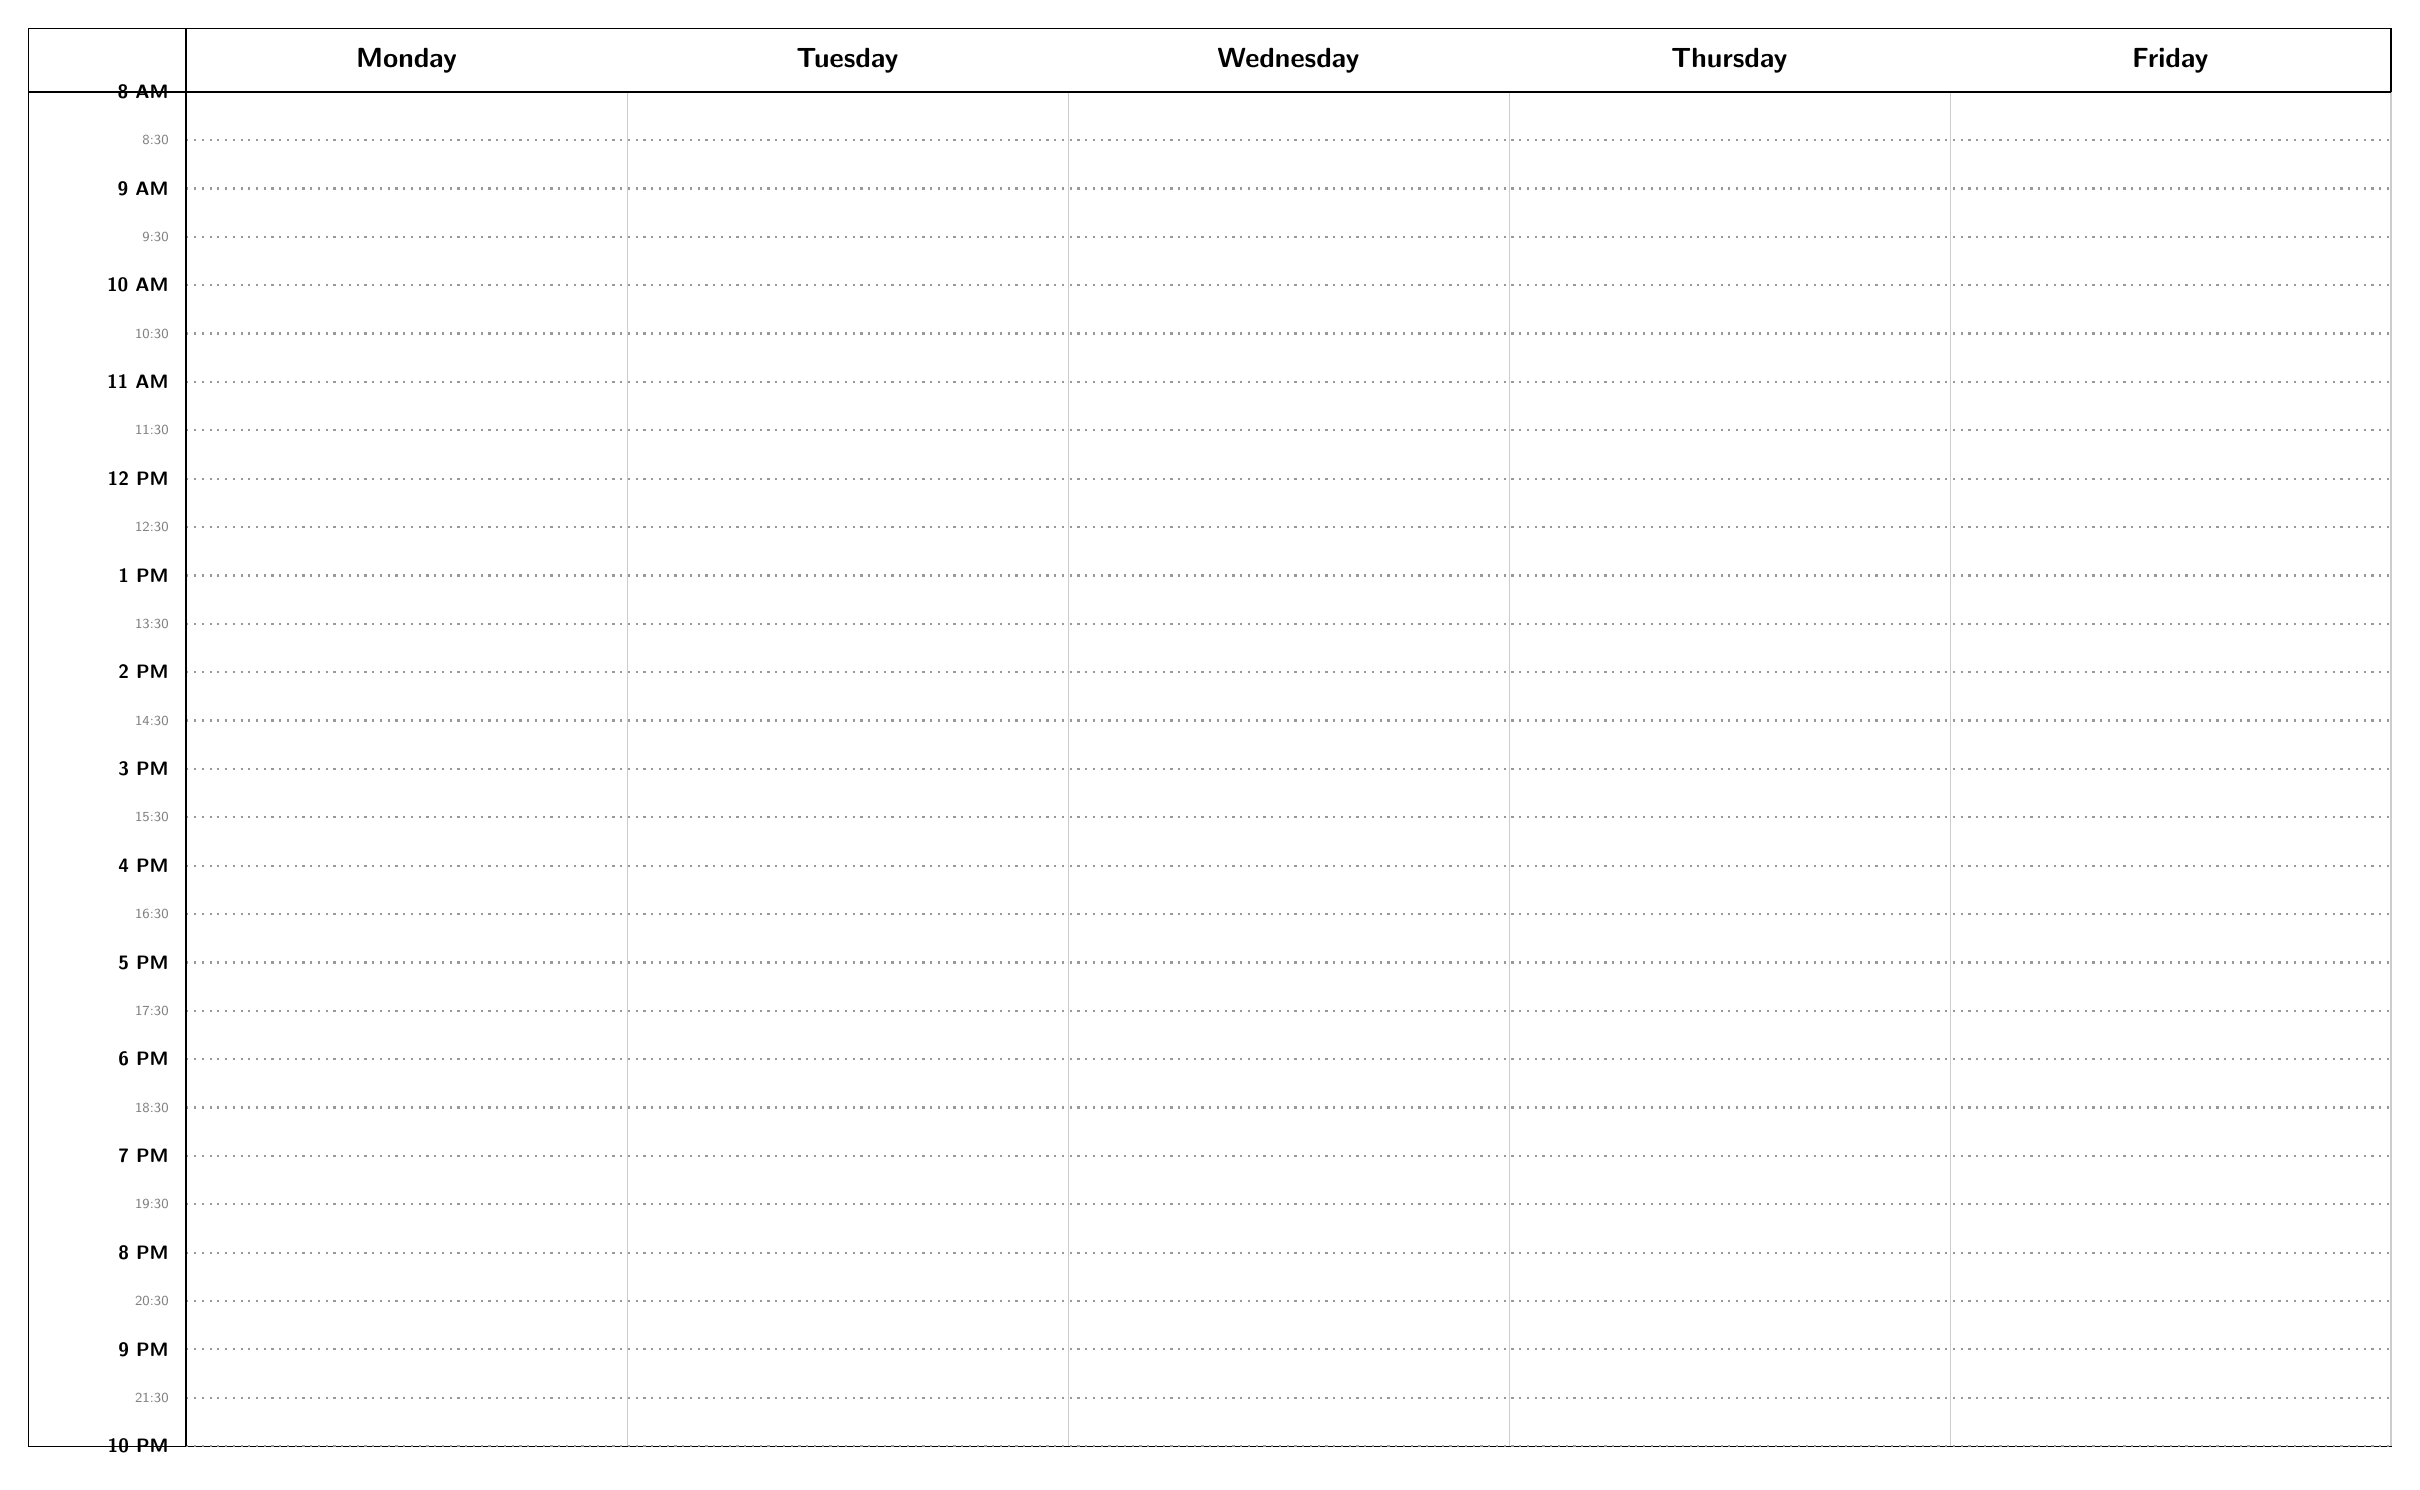
\begin{tikzpicture}
% Outline
\draw [draw=black] (0.0,0.0) rectangle (\D,\H);

% --- GRID AND TIME LABELS (30 min intervals) ---
% We loop through half-hours. Total hours * 2 = Total steps.
\def\totalsteps{\fpeval{(\hf-\hi)*2}}

\foreach \s in {0,...,\totalsteps}{
    % Current numerical time
    \def\curtime{\fpeval{\hi + \s/2}}
    % Y position calculation
    \def\y{\fpeval{\H - \h - (\curtime - \hi) * \dh}}
    
    % Draw horizontal line (Darker and dotted)
    \draw[dotted, black!40, line width=0.8pt] (\d, \y) -- (\D, \y);
    
    % Label Logic
    \def\hourpart{\fpeval{floor(\curtime)}}
    % Check if it is on the hour (integer) or half hour (.5)
    \ifnum\fpeval{round((\curtime - \hourpart)*10)}=5
        % It is XX:30
        \node[anchor=east, font=\tiny, gray] at (\d-0.1,\y) {\the\numexpr\hourpart\relax:30};
    \else
        % It is XX:00 -> Bold label
        \ifnum\hourpart>12
            \node[anchor=east, font=\scriptsize\bfseries] at (\d-0.1,\y) {\the\numexpr\hourpart-12\relax\ PM};
        \else
            \ifnum\hourpart=12
                \node[anchor=east, font=\scriptsize\bfseries] at (\d-0.1,\y) {12 PM};
            \else
                \node[anchor=east, font=\scriptsize\bfseries] at (\d-0.1,\y) {\hourpart\ AM};
            \fi
        \fi
    \fi
}

% --- HEADER DAYS ---
\foreach \j [count=\i] in \Days{
    % Calculate Center of Column
    % Start of column = \d + (\i-1)*\dd
    % Center = Start + \dd/2
    \def\x{\fpeval{\d + (\i - 1) * \dd + \dd/2}}
    \def\y{\fpeval{\H - \h/2}}
    \node[font=\bfseries] at (\x , \y)  {\j};
    % Draw vertical column separators
    \def\xline{\fpeval{\d + \i * \dd}}
    \draw[black!20] (\xline, 0) -- (\xline, \H-\h);
};

% Separator between Time and Monday
\draw[black, thick] (\d, 0) -- (\d, \H);
% Separator between Headers and Grid
\draw[black, thick] (0, \H-\h) -- (\D, \H-\h);


% ================= EVENTS =================

% --- MONDAY ---
\event[CMPE 212][Lecture][\LU][8.30][1][Watson 217][Sage];
\event[ELEC 274][Tutorial][\LU][9.30][1][Stirling B][TutColor];
\event[ENPH 239][Lecture][\LU][13.30][1][Stirling AUD][Sage];
% LAB: Mon Evening
\event[ELEC 274][Laboratory][\LU][18.30][3][Beamish-Munro 212 \\ \textbf{ONLY Wks 2,4,9,11}][LabColor];

% --- TUESDAY ---
\event[MTHE 212][Lecture][\MA][9.30][1][Jeffery 126][Sage];
\event[CMPE 212][Lecture][\MA][10.30][1][Watson 217][Sage];
\event[MTHE 281][Lecture][\MA][11.30][1][Stirling C][Sage];
\event[ELEC 274][Lecture][\MA][12.30][1][Kingston 201][Sage];
% LAB: Tues Afternoon
\event[CMPE 212][Laboratory][\MA][14.30][2][Kingston 209 \\ \textbf{Weekly} \\ (Except Wk 1,5,8,11)][LabColor];

% --- WEDNESDAY ---
\event[ENPH 239][Lecture][\ME][12.30][1][Stirling AUD][Sage];
\event[MTHE 281][Lecture][\ME][13.30][1][Stirling C][Sage];
\event[MTHE 212][Tutorial][\ME][14.30][1][Dunning 14][TutColor];
\event[MTHE 281][Tutorial][\ME][15.30][1][Stirling B][TutColor];

% --- THURSDAY ---
\event[MTHE 212][Lecture][\JE][8.30][1][Jeffery 126][Sage];
\event[CMPE 212][Lecture][\JE][9.30][1][Watson 217][Sage];
\event[ELEC 274][Lecture][\JE][11.30][1][Kingston 201][Sage];
\event[ENPH 239][Tutorial][\JE][14.30][1][Stirling AUD][TutColor];

% --- FRIDAY ---
\event[MTHE 212][Lecture][\VE][10.30][1][Jeffery 126][Sage];
\event[ENPH 239][Lecture][\VE][11.30][1][Stirling AUD][Sage];
\event[MTHE 281][Lecture][\VE][12.30][1][Stirling C][Sage];
\event[ELEC 274][Lecture][\VE][13.30][1][Kingston 201][Sage];

\end{tikzpicture}
\end{document}
